{\color{ggreen}\section{Regolarizzazione}}
\textcolor{ggreen}{\rule[5pt]{\textwidth}{1pt}}

\begin{wrapfigure}{r}{0.379\textwidth}
	\centering
	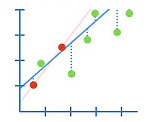
\includegraphics[width=0.370\textwidth]{IMMAGINI_RELAZIONE/Regolarizzazione.jpg}
\end{wrapfigure}

I metodi regolarizzati rinunciano a trovare la soluzione esatta del 
precedente problema di ottimizzazione, calcolando invece la soluzione di un problema leggermente "deviato",  
ovvero prendendo meno di riferimento il termine noto B che corrisponde all'immagine disturbata dal rumore. 
Quest’ultimo viene chiamato problema regolarizzato o regressione.
